\documentclass[output=paper]{langscibook} 

\author{Radek Šimík\affiliation{Charles University, Prague}\orcid{0000-0002-4736-195X} and Christoph Demian\affiliation{Humboldt-Universität zu Berlin}}
\title{Uniqueness and maximality in German and Polish: A production experiment}
\abstract{According to a prominent hypothesis word order manipulations in Slavic languages without articles can correspond to the use of definite or indefinite articles in languages that have them. We test this hypothesis using a production design in which participants build sentential picture descriptions from provided constituents. The crucial question is whether articles in German and word order in Polish are sensitive to visually depicted uniqueness or maximality of reference. We fail to find support for the article--word order correspondence; while the use of articles in German is sensitive to uniqueness/maximality, the use of word order in Polish is not.

\keywords{uniqueness, maximality, definiteness, articles, word order}}

\begin{document}
\maketitle

\section{Introduction}\label{sim-dem:sec:intro}

If a language lacks definite articles, call it an \textsc{articleless language}, does it also lack the semantics carried by definite articles? This question is standardly answered in the negative: articleless languages do not lack the pertinent semantics, they just have other formal means of expressing it (see e.g. \citealt{Kramsky1972}). This answer is in line with the common view that all languages are equal in their expressive capacity (e.g. \citealt{Aronoff2007}). The opposite view, namely that the lack of articles translates to the lack of article-related semantics, is a minor one, but it is not non-existent. \citet{Heim2011}, for instance, suggests that the semantics of bare NPs in languages without articles always corresponds to semantics of indefinites (existential and presupposition-free), no matter whether they correspond to (are translated by) definite or indefinite NPs in languages with this distinction.

The dominant tradition gave rise to a significant body of literature characterizing what we call here \textsc{definiteness correlates} (following \citealt{Simik.Demian2020}) -- morphological or syntactic devices whose semantics is claimed to correspond to definite articles. These devices include perfectivity (in its semantic impact on internal arguments; see \citealt{Krifka1989}; cf. \citealt{Filip1993,Filip1996}), topicality (whether manipulated by word order, prosody, subjecthood, or otherwise; see \citealt{Li.Thompson1976,Geist2010,Jenks2018}), certain types of adjectival declension (in Bosnian-Croatian-Serbian or Baltic languages; see \citealt{Hlebec1986,Progovac1998,Leko1999,Holvoet.Sprauniene2012,Serekaite2019}; cf. \citealt{Trenkic2004,Stankovic2015}), and others, such as grammatical number, classifiers, case-mark\-ing, or the position of NP-internal attributes.

In this paper we concentrate on word order as a definiteness correlate and test whether it has the capacity
to convey uniqueness or maximality, concepts that are commonly assumed to be conveyed by definite descriptions. The result of our production experiment does not support this hypothesis. Articles in German and word order in Polish behave very differently: while the former is sensitive to uniqueness and maximality, the latter is not. This result sheds doubt on the idea that the semantics of definiteness is universal.
It remains to be seen whether other concepts possibly conveyed by definite descriptions (such as referent identifiability) could be expressed by definiteness correlates in articleless languages.

The paper is organized as follows: \sectref{sim-dem:sec:wo} introduces the idea of word order being a definiteness correlate; \sectref{sim-dem:sec:exp} presents the experiment; \sectref{sim-dem:sec:concl} concludes the paper.

\section{Word order as a definiteness correlate}\label{sim-dem:sec:wo}

The consensus in the literature is that sentence-initial bare NPs in Slavic languages correspond to definite descriptions and are translated as such. Sentence-final bare NPs have either been considered indefinite or ambiguous/under\-speci\-fied. A few examples are provided below.

\ea\ea\gll Na stole je kniha.\\
on table is book\\
\glt `There is a book on the table.'
\ex\gll Kniha je na stole.\\
book is on table\\
\glt `The book is on the table.'\hfill (Czech; \citealt[42]{Kramsky1972})
\z\z

\ea\label{sim-dem:ex:rus1}\ea\gll Na stole stojala lampa.\\
on table stood lamp\\
\glt `There was a lamp on the desk.'
\ex\gll Lampa stojala na stole.\\
lamp stood on desk\\
\glt `The lamp was on a/the desk.'\hfill (Russian; \citealt[266]{Chvany1973})
\z\z

\ea\label{sim-dem:ex:pol1}\gll W pokoju siedziała dziewczyna.\\
in room sat girl\\
\glt `There was a girl sitting in the room.'
\ea\gll Wszedł chłopiec.\label{sim-dem:ex:pol1a}\\
entered boy\\
\glt `A boy entered.'
\ex\gll Chłopiec wszedł.\label{sim-dem:ex:pol1b}\\
boy entered\\
\glt `The boy entered.'\hfill (Polish; \citealt[215]{Szwedek1974a})
\z\z

\noindent Although the above observations are half a century old, similar ones have been reiterated and the idea of a more or less strict correspondence between word order and definiteness has gained the status of a truism (see e.g. \citealt{Szwedek1974}; \citeyear{Szwedek2011}; \citealt{Hlavsa1975}; \citealt{Birkenmaier1979}; \citealt{Gladrow1979,Gladrow1989,Weiss1983,Yokoyama1986,Hauenschild1993,Junghanns.Zybatow1997,Nesset1999,Leiss2000,Brun2001,Biskup2006,Kucerova2007,Kucerova2012,Topolinjska2009,Geist2010,Titov2012,Titov2017,Czardybon2017}; for a recent dissenting view see \citealt{Buncic2014}).

What is behind this word order--definiteness correspondence? For most researchers it is not word order alone that determines the interpretation. Sentence-initial, prosodically non-prominent bare NPs are considered topical (in the sense of aboutness topicality; \citealt{Reinhart1981}) and this property imposes a referential interpretation on bare NPs; the idea is that sentences can only be ``about'' referents and therefore cannot be quantificational (cf. \citealt{Endriss2009}). And while referential NPs can in principle be indefinite, particularly if they are ``specific'' (as in \citealt{Fodor.Sag1982}), a specific indefinite construal has been argued to be unavailable for bare NPs in articleless languages (\citealt{Dayal2004,Geist2010}; cf. \citealt{Borik2016,Borik.etal2020,Seres.Borik2020}). Referential bare NPs can thus only correspond to definites.

In formal Neo-Carlsonian approaches like \citeposst{Geist2010} (see \citealt{Chierchia1998} or \citealt{Dayal2004} for influential Neo-Carlsonian accounts), a bare NP like \textit{chłopiec} `boy' in \REF{sim-dem:ex:pol1}, starts its semantic life as a property -- \REF{sim-dem:ex:lex}, which, if used as an argument, can be type-shifted either to a \textsc{determinate} meaning -- \REF{sim-dem:ex:iota} -- or to an \textsc{indeterminate} meaning -- \REF{sim-dem:ex:ex}.\footnote{In the interest of clarity, we follow the terminological convention introduced in \citet{Coppock.Beaver2015}: the terms definite and indefinite refer solely to \textit{forms} -- NPs with definite and indefinite determiners, respectively, while the terms determinate and indeterminate refer to \textit{meanings} -- entities and existential quantifiers, respectively.}

\ea\ea \sib{chłopiec}${}=\lambda x[\textsc{boy}(x)]$\hfill lexical\label{sim-dem:ex:lex}
\ex \sib{chłopiec}${}=\iota x\,\textsc{boy}(x)$\hfill \textsc{iota-}shifted\label{sim-dem:ex:iota}
\ex \sib{chłopiec}${}=\lambda Q\exists x[\textsc{boy}(x)\wedge Q(x)]$\hfill \textsc{ex-}shifted\label{sim-dem:ex:ex}
\z\z

\noindent Type-shifting is a non-compositional semantic process which can be motivated or constrained by various factors. The primary motivation is a type-mismatch. In sentences \REF{sim-dem:ex:pol1a}/\REF{sim-dem:ex:pol1b}, \textit{chłopiec} is used as the argument of an intransitive verb, which is of type $\stb{e,t}$ and therefore expects an $e$-type expression as its argument. Since \textit{chłopiec} is lexically of type $\stb{e,t}$, it must shift. Both \textsc{iota}- and \textsc{ex}-shift will do; the former yields an expression of type $e$, the latter yields a quantifier (type $\stb{\stb{e,t},t}$) and the argument slot of the verb is filled by the $e$-type trace left behind by quantifier raising. Which type-shift is used is thus decided outside of the realm of semantics. According to \citet{Geist2010}, a sentence-final bare NP, as in \REF{sim-dem:ex:pol1a}, can be both determinate and indeterminate. A sentence-initial (prosodically non-prominent) bare NP, on the other hand, can only be determinate because the NP is topical and topical NPs must be referential (rather than quantificational).

In effect -- and that is important for our purposes -- the utterance in \REF{sim-dem:ex:pol1b} carries what is known as the \textsc{uniqueness presupposition}, the presupposition that there is exactly one boy (in some relevant evaluation situation). The presupposition is brought about by the \textsc{iota}-shift. The resulting semantics of \REF{sim-dem:ex:pol1a} is provided in \REF{sim-dem:ex:denot-initial}.

\ea \sib{Chłopiec wszedł} = \sib{The boy entered} = $\textsc{entered}\big(\iota x\,\textsc{boy}(x)\big)$\label{sim-dem:ex:denot-initial}\\
\textit{Presupposition:} There is exactly one boy (in the evaluation situation).
\z

\noindent The examples so far involved bare \textit{singular} NPs. There is little reason to assume, at least on the type of analysis proposed by \citet{Geist2010}, that they would behave differently from bare \textit{plural} NPs.\footnote{See \citet{Dayal2004}, who postulates an important difference between singulars and plurals. We set the issue aside here, but see \citet{Simik.Demian2020} for an experimental evaluation of \citeposst{Dayal2004} proposal.} Let us assume, for the sake of the argument, that the determinacy contrast is replicated in \REF{sim-dem:ex:plural} -- the sentence-initial NP corresponds to a definite NP in languages with articles and the sentence-final one to an indefinite (or more precisely bare) NP.

\ea\label{sim-dem:ex:plural}\ea\gll Weszli chłopcy.\label{sim-dem:ex:plural-a}\\
entered boys\\
\glt `Boys entered.'
\ex\gll Chłopcy weszli.\label{sim-dem:ex:plural-b}\\
boys entered\\
\glt `The boys entered.'\hfill (Polish)
\z\z

\noindent The determinate interpretation, implicated in \REF{sim-dem:ex:plural-b}, involves not the uniqueness presupposition, but rather the \textsc{maximality presupposition} -- the presupposition that there is a non-atomic entity containing all the atomic entities in the extension of `boy', what is called the \textsc{maximal plural entity} \citep{Sharvy1980,Link1983}. It is this entity that the determinate bare plural NP refers to. The semantics of \REF{sim-dem:ex:plural-b} is provided in \REF{sim-dem:ex:denot-initial-pl}.\footnote{In \citeposst{Link1983} formalism the formula $\sigma x\,P(x)$ indicates reference to the maximal plural entity in the extension of the plural predicate $\text{*}P$.}

\ea \sib{Chłopcy weszli} = \sib{The boys entered} = $\textsc{entered}\big(\sigma x\,\textsc{boy}(x)\big)$ \label{sim-dem:ex:denot-initial-pl}\\
\textit{Presupposition:} There is a maximal group of boys (in the evaluation situation).
\z

\noindent In summary, sentence-initial, prosodically non-prominent bare NPs in articleless languages are assumed to be topical and hence -- via referentiality -- correspond to definite NPs in languages with articles. This is what makes word order a definiteness correlate. In formal-semantic analyses like \citeposst{Geist2010}, the pertinent word order (and prosodic) configuration gives rise to a presupposition on a par with what definite NPs contribute, particularly the uniqueness presupposition (bare singulars) or the maximality presupposition (bare plurals). It is the presence of these presuppositions that we test in our experiment.

\section{Experiment}\label{sim-dem:sec:exp}

The goal of our experiment is to test the hypothesis that word order in articleless languages (here: Polish) can correspond to articles in languages that have them (here: German). The expectation is that word order production (in Polish) and article production (in German) will be affected by the uniqueness or maximality of reference. We will see that this expectation is borne out for article production but not for word order production, shedding doubt on the idea that word order is a definiteness correlate.

\subsection{Design}\label{sim-dem:sec:design}

We tested the impact of visually represented \textsc{uniqueness} and \textsc{maximality} (the main independent variables with binary values -- $\pm\textsf{uniq/max}$ -- and used for singulars and plurals, respectively) on the production of \textsc{word order} ($\textsf{subject}\prec\textsf{predicate}$ vs. $\textsf{predicate}\prec\textsf{subject}$) in Polish and \textsc{definiteness} ($\pm\textsf{definite}$) in German.\footnote{Throughout the paper, we type experimental variables in \textsc{small caps} and their levels in \textsf{sans-serif}.} We expect unique/maximal reference (as opposed to non-unique/non-maximal reference) to be matched by an increased proportion of definite description production in German and preverbal subject production in Polish. More particularly, we expect a higher proportion of $\textsf{subj}\prec\textsf{pred}$ order in the $+\textsf{uniq/max}$ condition; for German, we expect a higher proportion of $+\textsf{def}$ NPs in the $+\textsf{uniq/max}$ condition (both as compared to the $-\textsf{uniq/max}$ condition). The expectations are based on two hypothesized pressures governing the production. First, speakers are expected to prefer forms which are more expressive in terms of their presuppositions (in line with the Maximize Presupposition principle; \citealt{Heim1991}); this concerns the expected production of $+\textsf{def}$ (in German) and $\textsf{subj}\prec\textsf{pred}$ (in Polish) in the $+\textsf{uniq/max}$ condition. Second, speakers are expected to avoid forms which express presuppositions that are not supported in the situation; this concerns the expected production of $-\textsf{def}$ (in German) and $\textsf{pred}\prec\textsf{subj}$ (in Polish) in the $-\textsf{uniq/max}$ condition.

\begin{table}[t]
    \centering
    \begin{tabularx}{.8\textwidth}{rXXX}
    \lsptoprule
         &\textsc{uniq/max}&\textsc{number}&\textsc{conversation}\smallskip\\
         &within items&within items&within items\\
         &within subjects&within subjects&between subjects\smallskip\\
         &visual&linguistic&by instruction\\\midrule
         1&$+\textsf{unique}$&\textsf{singular}&$+\textsf{conversation}$\\
         2&$-\textsf{unique}$&\textsf{singular}&$+\textsf{conversation}$\\
         3&$+\textsf{maximal}$&\textsf{plural}&$+\textsf{conversation}$\\
         4&$-\textsf{maximal}$&\textsf{plural}&$+\textsf{conversation}$\\
         5&$+\textsf{unique}$&\textsf{singular}&$-\textsf{conversation}$\\
         6&$-\textsf{unique}$&\textsf{singular}&$-\textsf{conversation}$\\
         7&$+\textsf{maximal}$&\textsf{plural}&$-\textsf{conversation}$\\
         8&$-\textsf{maximal}$&\textsf{plural}&$-\textsf{conversation}$\\
    \lspbottomrule
    \end{tabularx}
    \caption{Manipulation of independent variables}
    \label{sim-dem:tab:factors}
\end{table}

The \textsc{uniq/max} manipulation correlated with \textsc{grammatical number} of the clausal subject: \textsc{uniqueness} was manipulated for \textsf{singular} subjects and \textsc{maximality} for \textsf{plural} ones. In addition, we included -- for exploratory reasons -- the binary variable \textsc{conversation} ($\pm\textsf{conversation}$). The variable was manipulated (between subjects) in the instructions to the experiment: the $+\textsf{conv}$ group received a brief instruction that they should imagine that they are looking at the visual stimulus together with a conversation partner and the description they produce is directed to her/him. The $-\textsf{conv}$ group did not receive this instruction; they were simply asked to provide a description of the visual stimulus.
% \largerpage

\begin{figure*}
\centering
%\begin{multicols}{2}
\fbox{\begin{subfigure}[t]{0.35\textwidth}
\centering
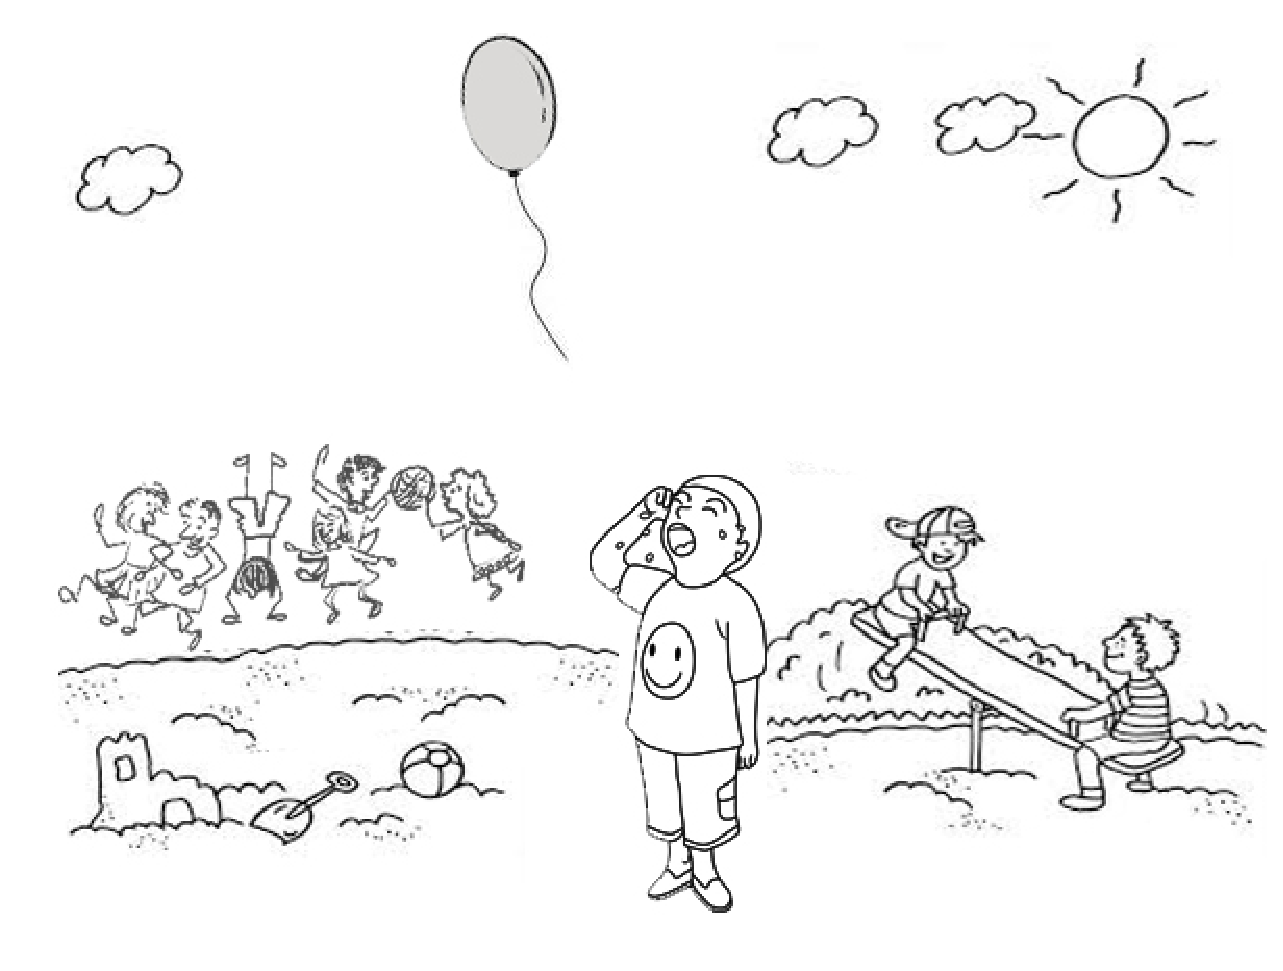
\includegraphics[scale=.2]{fig_balloon1.eps}
\caption{\textsf{sg $+$unique}}\label{sim-dem:fig:window-a}
\end{subfigure}}\hspace{.3cm}
~
\fbox{\begin{subfigure}[t]{0.35\textwidth}
\centering
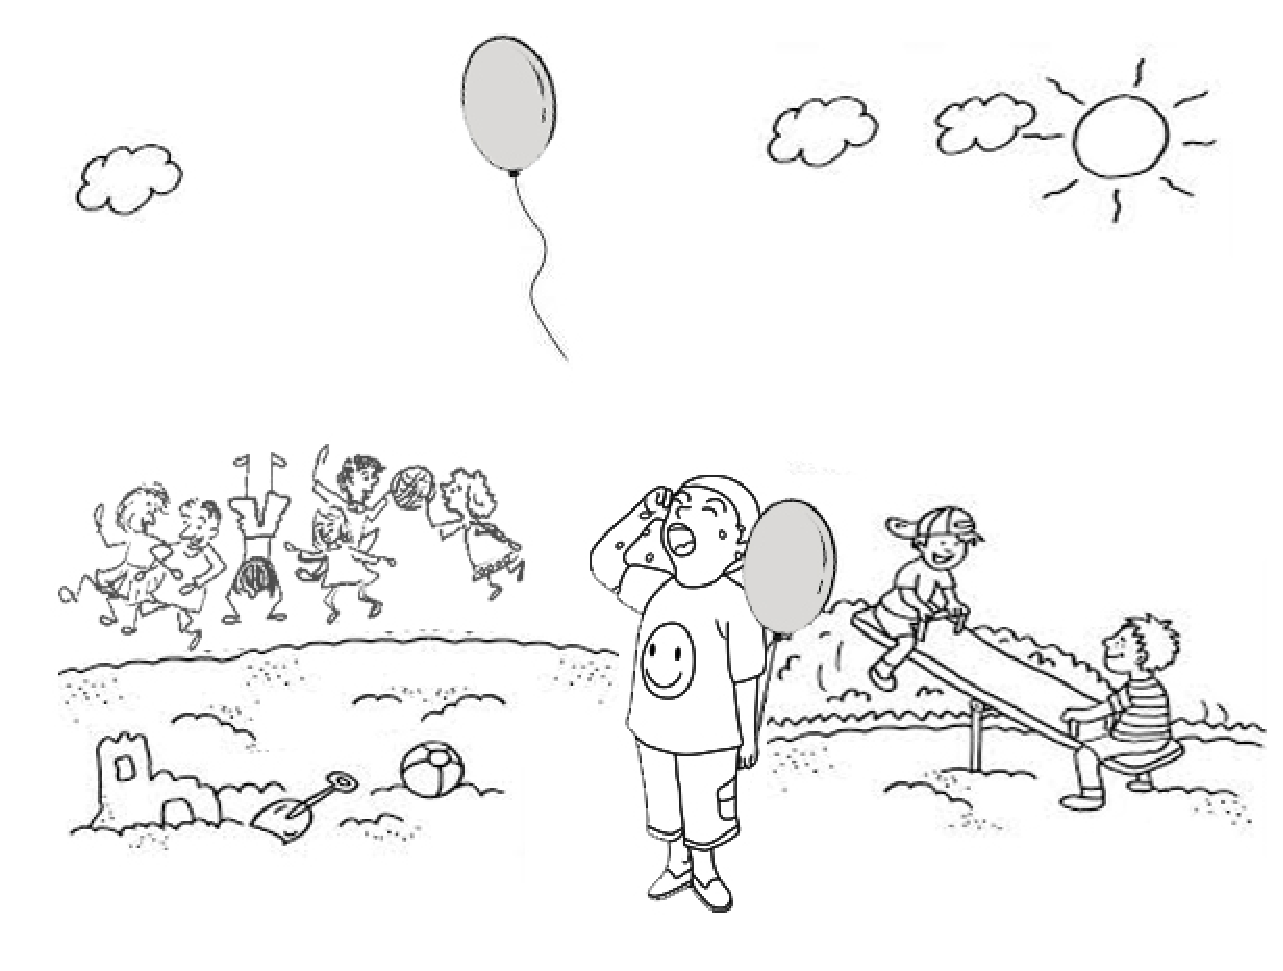
\includegraphics[scale=.2]{fig_balloon11.eps}
\caption{\textsf{sg $-$unique}}
\end{subfigure}}\vspace{.3cm}

\fbox{\begin{subfigure}[t]{0.35\textwidth}
\centering
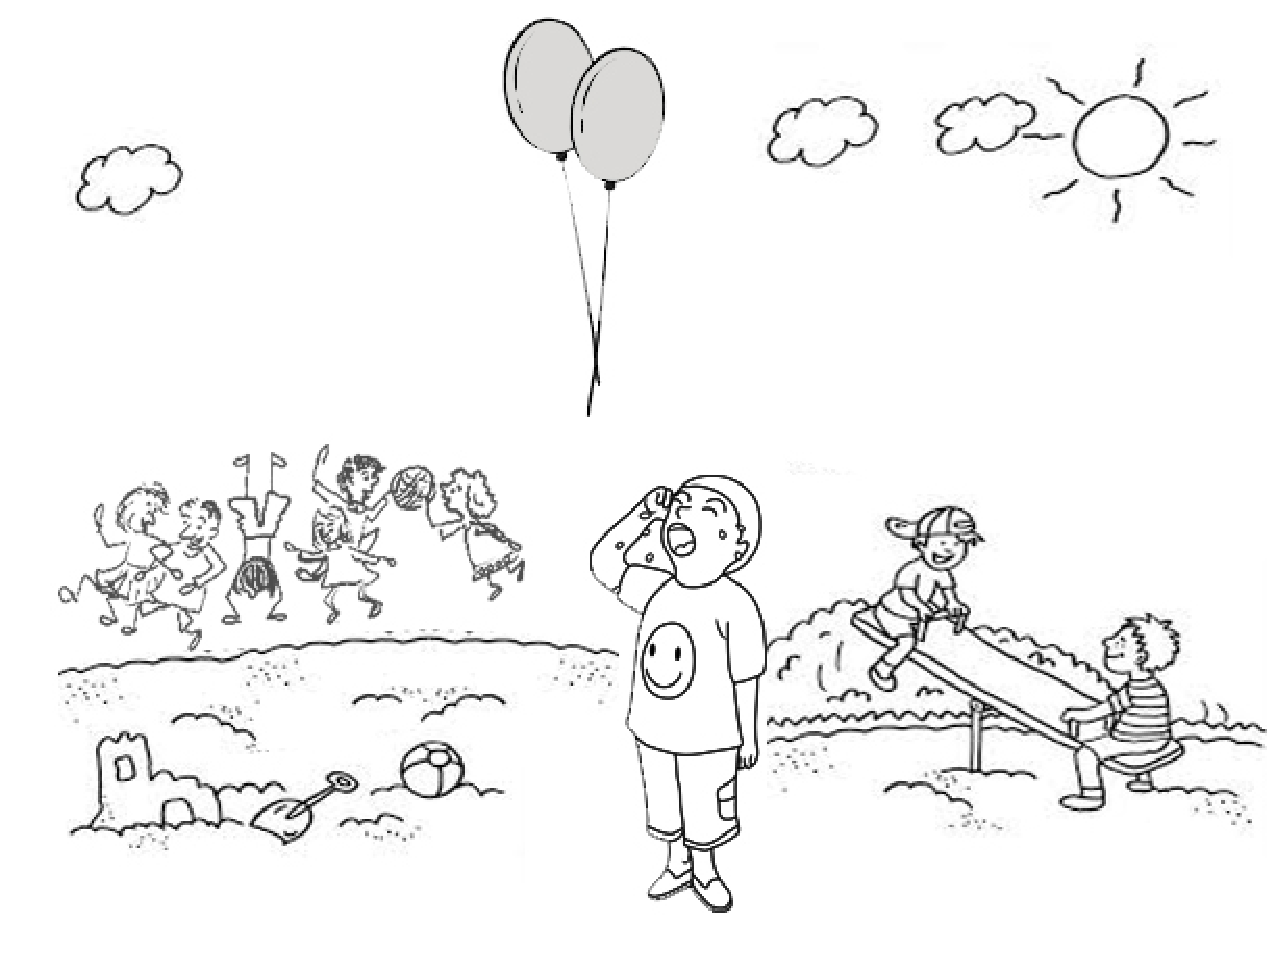
\includegraphics[scale=.2]{fig_balloon2.eps}
\caption{\textsf{pl $+$maximal}}
\end{subfigure}}\hspace{.3cm}
~
\fbox{\begin{subfigure}[t]{0.35\textwidth}
\centering
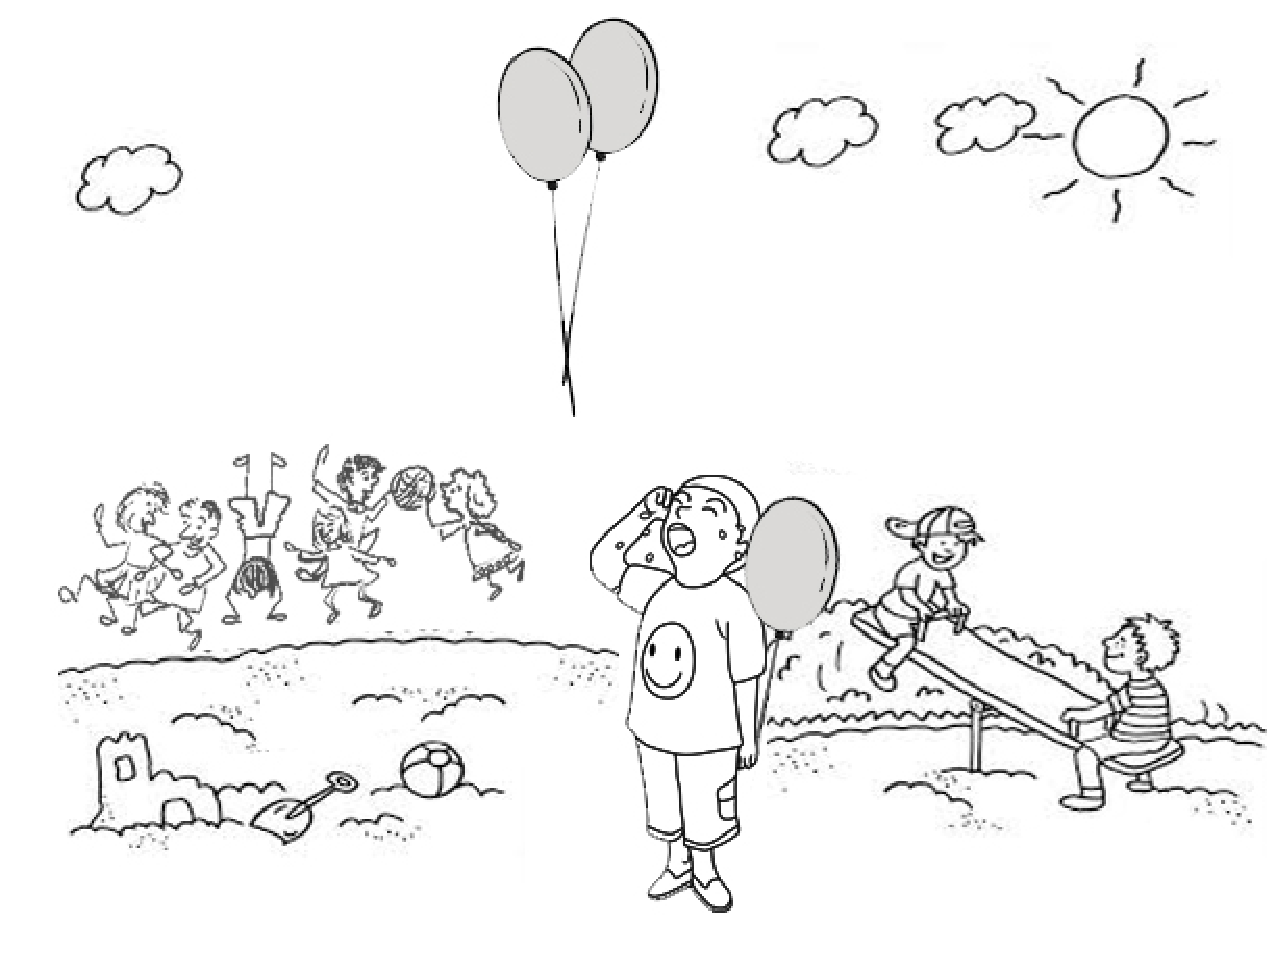
\includegraphics[scale=.2]{fig_balloon21.eps}
\caption{\textsf{pl $-$maximal}}\label{sim-dem:fig:window-d}
\end{subfigure}}
\caption{Visual part of token set of item 4 in both \textsc{uniq/max} conditions divided by \textsc{number}}\label{sim-dem:fig:window}
\end{figure*}

As summarized in \tabref{sim-dem:tab:factors}, the experiment involved a $2\times 2\times 2$ design, although the prediction only concerned the effect of \textsc{uniqueness/maximality}; \textsc{number} and \textsc{conversation} have been included for exploratory reasons.
% For this reason, the core statistical analysis only included \textsc{uniq/max} as predictor. Nevertheless, more complex models have also been fitted, esp. due to the large effect of \textsc{number} and its interaction with \textsc{uniq/max}.

\subsection{Materials, procedure, and participants}\label{sim-dem:sec:materials}

\largerpage %eventually to fit the whole of (8b-i) on page viii
We constructed 16 experimental items. The stimuli were selected and modified from \citet{Simik.Demian2020}.\footnote{All materials, experiment instructions, results, and analyses are available at \url{https://doi.org/10.17605/OSF.IO/KSTBZ}.} An example of a token set is provided in \figref{sim-dem:fig:window} (picture stimuli, manipulating \textsc{uniq/max}) and in \REF{sim-dem:ex:window} (linguistic building blocks, for Polish and German, respectively). The number of affected entities (here: balloons that flew away) always matched the grammatical number used in the building blocks (marked on nouns, predicates, or both). The picture and the building blocks were presented side-by-side, as illustrated in \figref{sim-dem:fig:pic-blocks}. The building blocks were pseudo-randomly distributed in a field, avoiding a bias in the ordering presented (in both left-right and top-down direction). There were two kinds of building blocks -- simple blocks, such as \fbox{\cnst{baloniki}}\,, and ``switch blocks'', such as \fbox{\cnst{mu} $\vert$ \cnst{jej}}\,, which presented the participants with a choice between two values.\footnote{One of the two values was pre-selected upon item presentation. Which value was pre-selected was pseudo-randomized and balanced across the experiment.} There were two kinds of operations available to the participants: (i) clicking on a switch block in order to switch the value of the block, whereby the selected value appeared on the top, on a white background; (ii) all blocks could be drag-and-dropped anywhere in the field.

\begin{figure}[t]
    \centering
    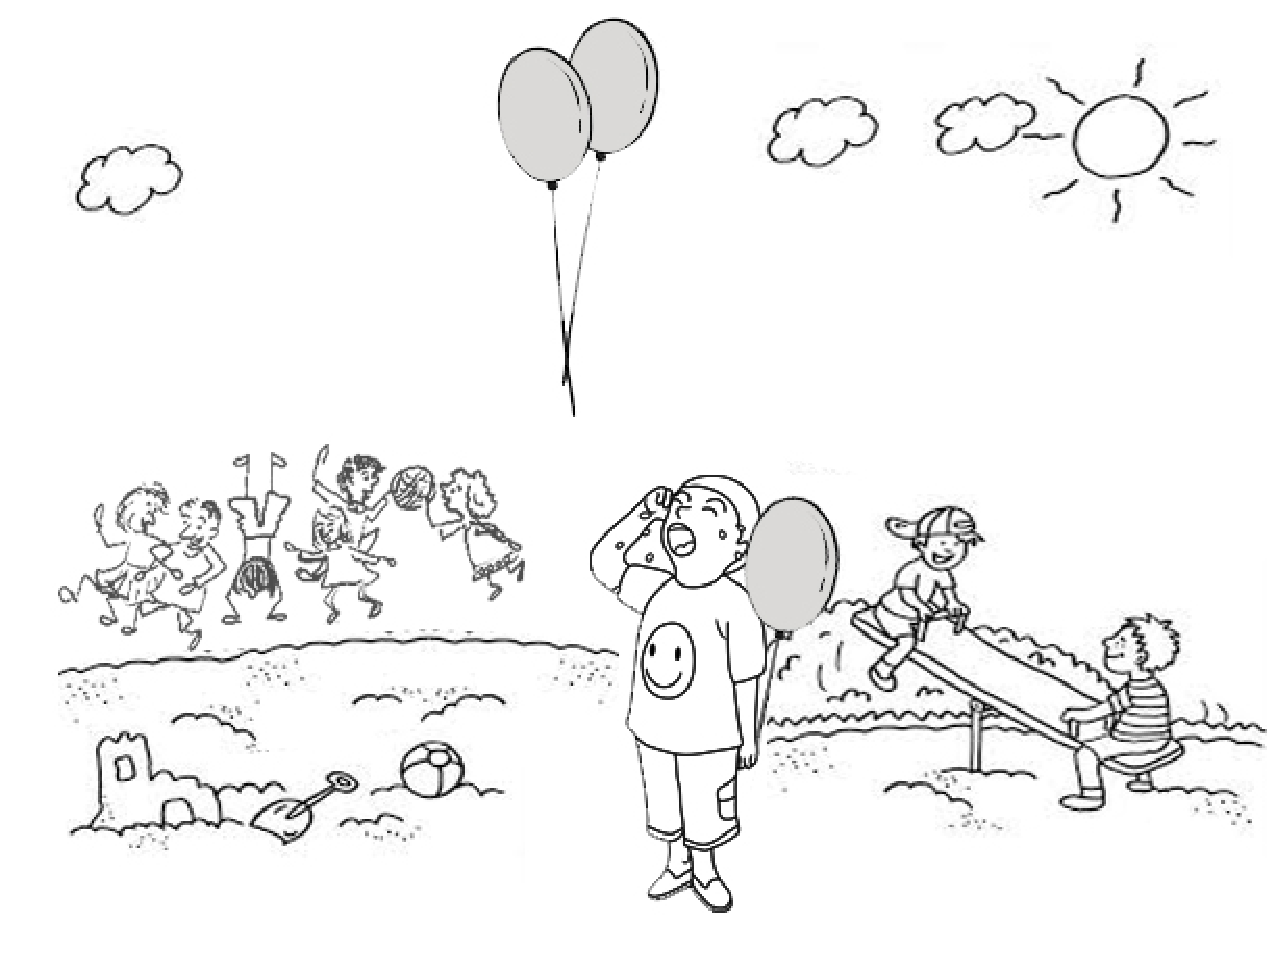
\includegraphics[scale=0.33]{fig_balloon21.eps} 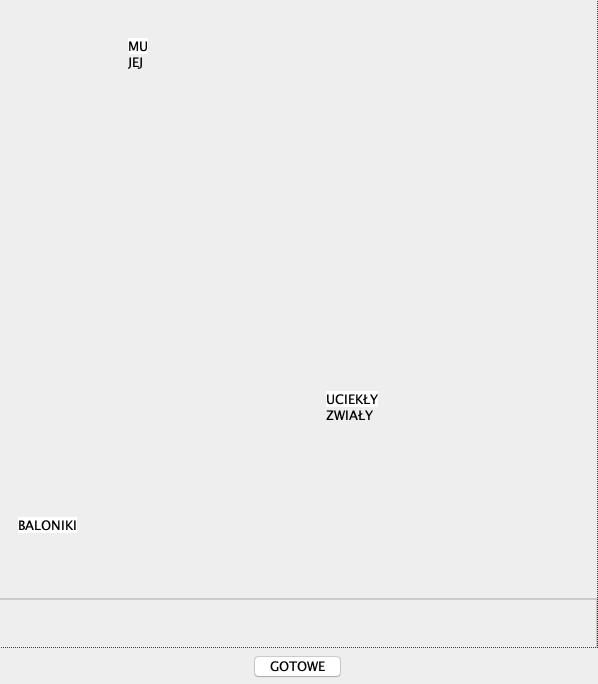
\includegraphics[scale=0.25]{prod_words.png}
    \caption{Presentation of item 4 in condition \textsf{pl $-$maximal} (Polish)}
    \label{sim-dem:fig:pic-blocks}
\end{figure}

\ea Linguistic part of token set of item 4 divided by \textsc{number}\label{sim-dem:ex:window}
\ea Polish
\ea\gll \fbox{\cnst{balonik}} \fbox{\cnst{mu $\vert$ jej}} \fbox{\cnst{uciekł $\vert$ zwiał}}\\
\hspace{4pt}balloon \hspace{4pt}{him $\vert$ her} \hspace{4pt}{escaped $\vert$ flew.away.\textsc{sg}}\\\hfill\textsf{sg}
\ex\gll \fbox{\cnst{baloniki}} \fbox{\cnst{mu $\vert$ jej}} \fbox{\cnst{uciekły $\vert$ zwiały}}\\
\hspace{4pt}balloons \hspace{4pt}{him $\vert$ her} \hspace{4pt}{escaped $\vert$ flew.away.\textsc{pl}}\\\hfill\textsf{pl}
\z
\ex German
\ea\gll \fbox{\cnst{der luftballon $\vert$ ein luftballon}} \fbox{\cnst{ist}} \fbox{\cnst{ihm $\vert$ ihr}} \fbox{\cnst{davongeflogen}}\\
\hspace{4pt}{the balloon $\vert$ a balloon} \hspace{4pt}\textsc{aux.sg} \hspace{4pt}{him $\vert$ her} \hspace{4pt}{flew.away}\\\hfill\textsf{sg}
\ex\gll \fbox{\cnst{die luftballons $\vert$ luftballons}} \fbox{\cnst{sind}} \fbox{\cnst{ihm $\vert$ ihr}}\hspace{.5cm} \fbox{\cnst{davongeflogen}}\\
\hspace{4pt}{the balloons $\vert$ balloons} \hspace{4pt}\textsc{aux.pl} \hspace{4pt}{him $\vert$ her} \hspace{4pt}{flew.away}\\\hfill\textsf{pl}
\z
\z\z

\noindent The task of the participant was to produce a description of the picture, selecting the appropriate values (by clicking on switch blocks), and ordering the blocks one after another in the pane located in the bottom part of the field (by drag-and-dropping). The participants indicated that they are finished by clicking on the \fbox{\cnst{gotowe}} / \fbox{\cnst{fertig}} (`done') button located below the target pane.

\largerpage[-1] % to push first line of (9a) to page xi
Both the German and the Polish version of the experiment made use of both operations -- switching block values and drag-and-dropping. In German, the target value of the dependent variable (\textsc{definiteness}) was achieved by switching block values; in Polish, the target value of the dependent variable (\textsc{word order}) was achieved by drag-and-dropping. The operations not essential for the core measure (drag-and-dropping in German, switching non-essential values in both German and Polish) had two functions: bringing the two language versions closer together and distracting the participants from the experimental manipulation. The distractor switches typically involved either synonyms (making the choice non-essential) or a clear match vs. clear mismatch (making the choice easy).

With a single exception, all the experimental items involved intransitive predications, which readily allow for both subject $\prec$ predicate and predicate $\prec$ subject orders in all new contexts in Slavic languages \citep{Junghanns2002}. Word order was thus free to be used for other than information-structural purposes.

Apart from the 16 critical items, one of which has just been exemplified, the design involved 32 filler items (partly containing additional miniexperiments). All the items were distributed in multiple versions of the experiment following the Latin square design. Each participant saw exactly one token from each item, more particularly 8 items in the \textsf{$+$unique/maximal} condition and 8 in the \textsf{$-$unique/maximal} condition.

The analyzed dataset contained data from 29 Polish participants (students from Wrocław) and from 15 German participants (students from Berlin). The intention was to have 32 Polish and 16 German participants, in order to have the same number of data-points for each individual condition.\footnote{The reason for a larger number of Polish participants is that we expected the effect of \textsc{uniq/max} to be less robust in Polish than in German. These expectations are based on the effect sizes found in \citet{Simik.Demian2020}.\label{sim-dem:fn:effect-size}} One German and one Polish participant were missing for technical reasons. Two Polish participants were excluded from the dataset because of low data quality; one formed more than 3 ungrammatical sentences and both never used the switch function, suggesting the lack of attention or non-cooperative behavior. The German participants received a compensation of €5; the Polish participants did the experiment as part of their course requirement.

The experiment was presented in computer pools within scheduled sessions, using Java-based software developed by one of the authors. The experiment itself was preceded by instructions (which included the manipulation of the \textsc{conversation} variable, as described above) and by an act-out illustration of the procedure, in which the participants were forced to make use of both operations -- switching the value of switch blocks and drag-and-dropping. There was no time limit. Most participants completed the experiment in 20--30 minutes.

\subsection{Predictions and results}

\subsubsection{Effect of \textsc{uniq/max}}
\largerpage[-1] % to push first line of (9a) to page xi

The sentences in \REF{sim-dem:ex:outcome} illustrate the possible grammatical outcomes of the Polish and German version of item 4 in the \textsf{singular} condition.\footnote{Ungrammatical outcomes such as \textit{*się okno zbiło} in Polish or \textit{*das Fenster zerbrochen ist} in German were possible but extremely rare (in Polish) and not attested (in German).}

\ea\label{sim-dem:ex:outcome}\ea Polish
\ea\gll Balonik mu zwiał.\\
balloon him flew.away.\textsc{sg}\\\hfill $\textsf{subj}\prec\textsf{pred}$
\glt By hypothesis: `The balloon flew away (from him).'
\ex\gll Zwiał mu balonik.\\
flew.away.\textsc{sg} him balloon\\\hfill $\textsf{pred}\prec\textsf{subj}$
\glt By hypothesis: `A balloon flew away (from him).'
\z
\ex German
\ea\gll Der Luftballon ist ihm davongeflogen.\\
the balloon is.\textsc{aux} him flew.away\\\hfill$+\textsf{definite}$
\glt `The balloon flew away (from him).'
\ex\gll Ein Luftballon ist ihm davongeflogen.\\
a balloon is.\textsc{aux} him flew.away\\\hfill$-\textsf{definite}$
\glt `A balloon flew away (from him).'
\z
\z\z

\noindent\figref{sim-dem:fig:prediction} illustrates the predicted main effect of the \textsc{uniq/max} variable on the \textsc{word order} in Polish and \textsc{definiteness} in German.\footnote{The absolute numbers (set to $0.8$ and $0.3$) are immaterial in these diagrams, what is important is the differing proportion. Although we expect the effect size to be smaller in Polish than in German (cf. footnote \ref{sim-dem:fn:effect-size}), this expectation is only based on previous experimental results \citep{Simik.Demian2020} and is not theoretically grounded. That is why we do not encode it in the visualization of the prediction.\label{sim-dem:fn:prediction}} In Polish, we expect a higher proportion of $\textsf{subject}\prec\textsf{predicate}$ outcomes in the $+\textsf{uniq/max}$ condition than in the $-\textsf{uniq/max}$ condition. Analogously, in German, we expect a higher proportion of $+\textsf{definite}$ outcomes in $+\textsf{uniq/max}$ condition than in the $-\textsf{uniq/max}$ condition.

%prediction fig

\begin{figure}
\begin{subfigure}[t]{0.48\textwidth}
\centering
  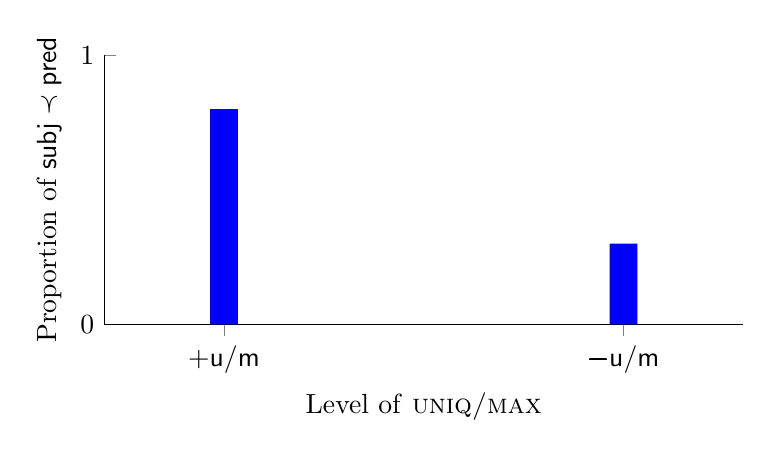
\begin{tikzpicture}
    \begin{axis}[
	xlabel={Level of \textsc{uniq/max}},  
	ylabel={Proportion of $\textsf{subj}\prec\textsf{pred}$}, 
	axis lines*=left, 
        width  = .8\textwidth,
	height = 5cm,
    % 	nodes near coords, 
    % 	nodes near coords style={text=black},
    % 	every node near coord/.append style={font=\tiny},
        % nodes near coords align={vertical},
	ymin=0,
	ymax=1,
% 	xmax=100,
    xtick=data,
	ytick distance=1,
	ylabel near ticks,
 	x tick label style={font=\sffamily},
	ybar,
	enlarge x limits=0.3,
	symbolic x coords={+u/m, \textminus u/m},
	]
	\addplot[fill=blue,draw=none] coordinates {
	    (+u/m,0.8)
        (\textminus u/m,0.3)
	}; 
    \end{axis} 
  \end{tikzpicture} 
\caption{Polish}\label{sim-dem:fig:predictions-polish}
\end{subfigure}
~
\begin{subfigure}[t]{0.48\textwidth}
\centering
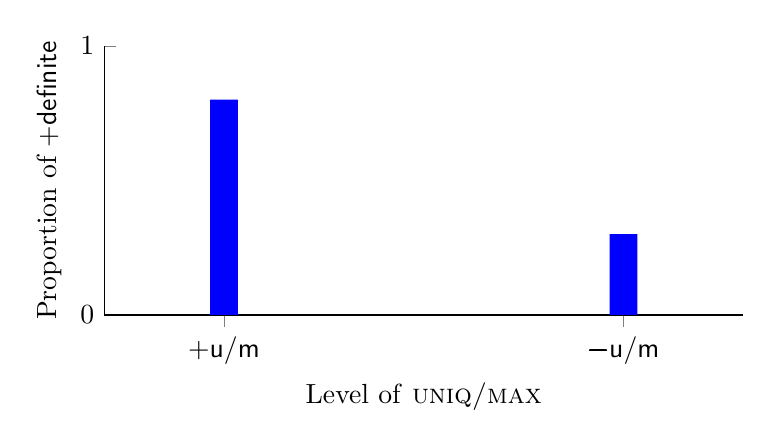
\begin{tikzpicture}
    \begin{axis}[
	xlabel={Level of \textsc{uniq/max}},  
	ylabel={Proportion of $+\textsf{definite}$}, 
	axis lines*=left, 
        width  = .8\textwidth,
	height = 5cm,
    % 	nodes near coords, 
    % 	nodes near coords style={text=black},
    % 	every node near coord/.append style={font=\tiny},
        % nodes near coords align={vertical},
	ymin=0,
	ymax=1,
	ytick distance=1,
	xtick=data,
	ylabel near ticks,
	x tick label style={font=\sffamily},
	ybar,
	enlarge x limits=0.3,
	symbolic x coords={+u/m, \textminus u/m},
	]
	\addplot[fill=blue,draw=none] coordinates {
	    (+u/m,0.8)
        (\textminus u/m,0.3)
	}; 
    \end{axis} 
  \end{tikzpicture}
\caption{German}
\end{subfigure}
    \caption{Prediction: Main effect of \textsc{uniq/max} on \textsc{word order} in Polish and \textsc{definiteness} in German}
    \label{sim-dem:fig:prediction}
\end{figure}

Figures \ref{sim-dem:fig:result-main}--\ref{sim-dem:fig:result-conv} show the results.\footnote{Data from 2 items (3 and 8) have been excluded from the Polish dataset (post-hoc) because of aspects of the language--picture correspondence which (might have) affected the critical manipulation. In addition, 6 datapoints have been excluded from the Polish dataset because they were ungrammatical.\label{sim-dem:fn:excluded-items}} We first discuss them informally, based on the visual inspection of the figures, and then turn to statistical models. As is evident from \figref{sim-dem:fig:result-main}, Polish participants mostly produced the $\textsf{subj}\prec\textsf{pred}$ order, independently of the \textsc{uniq/max} manipulation. German participants were sensitive to the \textsc{uniq/max} manipulation: they produced significantly more $+\textsf{definite}$ NPs if the picture they described satisfied uniqueness or maximality (\textsf{$+$u/m}) than if it did not (\textsf{$-$u/m}). Figures \ref{sim-dem:fig:result-num} and \ref{sim-dem:fig:result-conv} show the results divided by \textsc{number} and by \textsc{conversation}, respectively. What is most clearly visible is the effect of \textsc{number} in German, where definite NPs were used much more in the \textsf{plural} than in the \textsf{singular}. At the same time, there appears to be an interaction between \textsc{number} and \textsc{uniq/max}: the expected effect of \textsc{uniq/max} (more $+\textsf{definite}$ NPs in $+\textsf{u/m}$) is much more clearly pronounced in the \textsf{singular} than in the \textsf{plural} condition. In Polish, the impact of both \textsc{number} and \textsc{conversation} is rather subtle.

%main result fig
\begin{figure}
\begin{subfigure}[t]{0.48\textwidth}
\centering
  \begin{tikzpicture}
    \begin{axis}[
	xlabel={Level of \textsc{uniq/max}},  
	ylabel={Proportion of $\textsf{subj}\prec\textsf{pred}$}, 
    % ylabel={a,b},
    	nodes near coords, 
    % 	nodes near coords style={text=black},
        every node near coord/.append style={font=\tiny},
        nodes near coords align={vertical},
	axis lines*=left, 
        width  = .8\textwidth,
	height = 5cm,
	ymin=0,
	ymax=1,
	ytick distance=.2,
	xtick=data,
	ylabel near ticks,
	x tick label style={font=\sffamily},
	ybar,
	enlarge x limits=0.3,
	symbolic x coords={+u/m, \textminus u/m},
    % symbolic x coords={a,b},
	]
	\addplot[fill=red,draw=none] coordinates {
	    (+u/m,0.85)
        (\textminus u/m,0.86)
	}; 
    \end{axis} 
  \end{tikzpicture} 
\caption{Polish}%\label{sim-dem:fig:results-polish}
\end{subfigure}
~
\begin{subfigure}[t]{0.48\textwidth}
\centering
\begin{tikzpicture}
    \begin{axis}[
	xlabel={Level of \textsc{uniq/max}},  
	ylabel={Proportion of $+\textsf{definite}$}, 
	axis lines*=left, 
        width  = .8\textwidth,
	height = 5cm,
    	nodes near coords, 
    % 	nodes near coords style={text=black},
        every node near coord/.append style={font=\tiny},
        nodes near coords align={vertical},
	ymin=0,
	ymax=1,
	ytick distance=.2,
	xtick=data,
	ylabel near ticks,
	x tick label style={font=\sffamily},
	ybar,
	enlarge x limits=0.3,
	symbolic x coords={+u/m, \textminus u/m},
	]
	\addplot[fill=red,draw=none] coordinates {
	    (+u/m,0.82)
        (\textminus u/m,0.39)
	}; 
    \end{axis} 
  \end{tikzpicture}
\caption{German}
\end{subfigure}
    \caption{Result}
    \label{sim-dem:fig:result-main}
\end{figure}

%number result fig
\begin{figure}
\begin{subfigure}[t]{0.48\textwidth}
\raggedright
  \begin{tikzpicture}
    \begin{axis}[
	xlabel={Level of \textsc{uniq/max}},  
	ylabel={Proportion of $\textsf{subj}\prec\textsf{pred}$}, 
	axis lines*=left, 
        width  = .8\textwidth,
	height = 5cm,
    	nodes near coords, 
    % 	nodes near coords style={text=black},
    	every node near coord/.append style={font=\tiny},
        nodes near coords align={vertical},
	ymin=0,
	ymax=1,
	ytick distance=.2,
	xtick=data,
	ylabel near ticks,
	x tick label style={font=\sffamily},
	ybar=5pt,
	legend pos=outer north east,
	enlarge x limits=0.3,
	symbolic x coords={+u/m, \textminus u/m},
	]
	\addplot[fill=red!30,draw=none] coordinates {
	    (+u/m,0.91)
        (\textminus u/m,0.84)
	};
	\addplot[fill=red,draw=none] coordinates {
	    (+u/m,0.80)
        (\textminus u/m,0.87)
	};
	\legend{\textsf{sg}, \textsf{pl}}
    \end{axis} 
  \end{tikzpicture} 
\caption{Polish}%\label{sim-dem:fig:result-polish}
\end{subfigure}
~
\begin{subfigure}[t]{0.48\textwidth}
\raggedleft
\begin{tikzpicture}
    \begin{axis}[
	xlabel={Level of \textsc{uniq/max}},  
	ylabel={Proportion of $+\textsf{definite}$}, 
	axis lines*=left, 
        width  = .8\textwidth,
	height = 5cm,
    	nodes near coords, 
    % 	nodes near coords style={text=black},
        every node near coord/.append style={font=\tiny},
        nodes near coords align={vertical},
	ymin=0,
	ymax=1,
	ytick distance=.2,
	xtick=data,
	ylabel near ticks,
	x tick label style={font=\sffamily},
	ybar=5pt,
	legend pos=outer north east,
	enlarge x limits=0.3,
	symbolic x coords={+u/m, \textminus u/m},
	]
	\addplot[fill=red!30,draw=none] coordinates {
	    (+u/m,0.72)
        (\textminus u/m,0.10)
	};
	\addplot[fill=red,draw=none] coordinates {
	    (+u/m,0.92)
        (\textminus u/m,0.68)
	};
	\legend{\textsf{sg}, \textsf{pl}} 
    \end{axis} 
  \end{tikzpicture}
\caption{German}
\end{subfigure}
    \caption{Results divided by \textsc{number}}
    \label{sim-dem:fig:result-num}
\end{figure}

%conv result fig
\begin{figure}
\begin{subfigure}[t]{0.48\textwidth}
\raggedright
  \begin{tikzpicture}
    \begin{axis}[
	xlabel={Level of \textsc{uniq/max}},  
	ylabel={Proportion of $\textsf{subj}\prec\textsf{pred}$}, 
	axis lines*=left, 
        width  = .8\textwidth,
	height = 5cm,
    	nodes near coords, 
    % 	nodes near coords style={text=black},
        every node near coord/.append style={font=\tiny},
        nodes near coords align={vertical},
	ymin=0,
	ymax=1,
	ytick distance=.2,
	xtick=data,
	ylabel near ticks,
	x tick label style={font=\sffamily},
	ybar=5pt,
	legend pos=outer north east,
	enlarge x limits=0.3,
	symbolic x coords={+u/m, \textminus u/m},
	]
	\addplot[fill=red!30,draw=none] coordinates {
	    (+u/m,0.91)
        (\textminus u/m,0.89)
	};
	\addplot[fill=red,draw=none] coordinates {
	    (+u/m,0.80)
        (\textminus u/m,0.83)
	};
	\legend{\textsf{$+$conv}, \textsf{$-$conv}}
    \end{axis} 
  \end{tikzpicture} 
\caption{Polish}%\label{sim-dem:fig:predictions-polish}
\end{subfigure}
~
\begin{subfigure}[t]{0.48\textwidth}
\raggedleft
\begin{tikzpicture}
    \begin{axis}[
	xlabel={Level of \textsc{uniq/max}},  
	ylabel={Proportion of $+\textsf{definite}$}, 
	axis lines*=left, 
        width  = .8\textwidth,
	height = 5cm,
    	nodes near coords, 
    % 	nodes near coords style={text=black},
        every node near coord/.append style={font=\tiny},
        nodes near coords align={vertical},
	ymin=0,
	ymax=1,
	ytick distance=.2,
	xtick=data,
	ylabel near ticks,
	x tick label style={font=\sffamily},
	ybar=5pt,
	legend pos=outer north east,
	enlarge x limits=0.3,
	symbolic x coords={+u/m, \textminus u/m},
	]
	\addplot[fill=red!30,draw=none] coordinates {
	    (+u/m,0.80)
        (\textminus u/m,0.36)
	};
	\addplot[fill=red,draw=none] coordinates {
	    (+u/m,0.83)
        (\textminus u/m,0.42)
	};
	\legend{\textsf{$+$conv}, \textsf{$-$conv}} 
    \end{axis} 
  \end{tikzpicture}
\caption{German}
\end{subfigure}
    \caption{Results divided by \textsc{conversation}}
    \label{sim-dem:fig:result-conv}
\end{figure}

We fitted a number of generalized linear mixed-effects models, using the \texttt{glmer} function from the \texttt{lme4} package \citep{Bates.etal2015} of R \citep{RCore2017}.

For Polish, models in which \textsc{uniq/max}, \textsc{number}, and \textsc{conversation} were all combined did not converge. Therefore, we fitted two less complex models -- one with \textsc{uniq/max} and \textsc{number} as predictors (see \tabref{sim-dem:tab:stats3pl}) and the other with \textsc{uniq/max} and \textsc{conversation} as predictors (see \tabref{sim-dem:tab:stats4pl}). The predictors were sum coded and random intercepts for subjects and items have been included. Neither of the two models reveal the expected main effect of \textsc{uniq/max} ($z=0.207$, $z=-0.064$, respectively, both $p\text{s}>0.8$). The model with \textsc{number} reveals a weak interaction between \textsc{uniq/max} and \textsc{number} ($z=-2.281,p=0.023$) and the model with \textsc{conversation} reveals a weak main effect of this factor ($z=2.497,p=0.013$), suggesting that $+\textsf{conv}$ yielded significantly more $\textsf{subj}\prec\textsf{pred}$ orders than $-\textsf{conv}$.

For German, we fitted a model with \textsc{uniq/max}, \textsc{number}, and \textsc{conversation} as predictors. The predictors were sum coded and included a random intercept for items (see \tabref{sim-dem:tab:stats3ge}); the more complex model with intercepts for items and subjects did not converge. The model reveals the expected main effect of \textsc{uniq/max} ($z=6.071,p<0.001$): more $+\textsf{definite}$ were produced in the $+\textsf{uniq/max}$ condition than in the $-\textsf{uniq/max}$ condition. Additionally, a main effect of \textsc{number} was found ($z=5.719,p<0.001$; more $+\textsf{definite}$ were produced in the \textsf{plural} condition than in the \textsf{singular} condition) and, finally, an interaction between \textsc{uniq/max} and \textsc{number} was found ($z=-2.211,p=0.03$; a much more pronounced effect of \textsc{uniq/max} in \textsf{singular} than in \textsf{plural}.

% The models predicted the $\textsf{subj}\prec\textsf{pred}$ response for Polish and the $+\textsf{def}$ response for German as a function of \textsc{uniq/max} (baseline: $+\textsf{u/m}$) and included random intercepts for subjects and items. The model for German revealed an effect of \textsc{uniq/max} on \textsc{definiteness} (\tabref{sim-dem:tab:stats1ge}); the model for Polish revealed no effect of \textsc{uniq/max} on \textsc{word order} (\tabref{sim-dem:tab:stats1pl}).

%stats3pl
\begin{table}
    \centering
    \begin{tabular}{lrrrr}
    \lsptoprule
\textbf{Fixed effects}&\\\midrule
&            Estimate & SE & $z$ value & $p$ value\\  
Intercept               &$-3.8608$   &$0.9963$ &$-3.875$  &$<0.001$\\
\textsc{uniq/max}       &$0.0406$  &$0.1959$ &$0.207$ &$0.84$\\
\textsc{number}         &$0.2898$  &$0.1994$ &$1.454$ &$0.15$\\
\textsc{uniq/max*num}&$-0.4572$  &$0.2005$ &$-2.281$ &$0.023$\medskip\\
\textbf{Random effects}&\\\midrule
& Variance &SD\\
subject&$1.184$&$1.088$\\
item&$7.082$&$2.661$\\
\lspbottomrule
    \end{tabular}
    \caption{Generalized linear mixed model fit by maximum likelihood (Laplace Approximation) for Polish ($N=400$; predictors: \textsc{uniq/max} and \textsc{number}; log-likelihood: $-115.5$)}
    \label{sim-dem:tab:stats3pl}
\end{table}

%stats4pl
\begin{table}
    \begin{tabular}{lrrrr}
    \lsptoprule
\textbf{Fixed effects}&\\\midrule
&            Estimate & SE & $z$ value & $p$ value\\  
Intercept               &$-3.6824$   &$0.9366$ &$-3.932$  &$<0.001$\\
\textsc{uniq/max}       &$-0.0124$  &$0.1930$ &$-0.064$ &$0.95$\\
\textsc{conv}         &$0.6088$  &$0.2438$ &$2.497$ &$0.013$\\
\textsc{uniq/max*conv}&$-0.0188$  &$0.7858$ &$-0.024$ &$0.98$\medskip\\
\textbf{Random effects}&\\\midrule
& Variance &SD\\
subject&$0.574$&$0.758$\\
item&$6.548$&$2.559$\\
\lspbottomrule
    \end{tabular}
    \caption{Generalized linear mixed model fit by maximum likelihood (Laplace Approximation) for Polish ($N=400$; predictors: \textsc{uniq/max} and \textsc{conversation}; log-likelihood: $-116.2$)}
    \label{sim-dem:tab:stats4pl}
\end{table}

%stats3ge
\begin{table}
    \begin{tabular}{lrrrr}
    \lsptoprule
\textbf{Fixed effects}&\\\midrule
&            Estimate & SE & $z$ value & $p$ value\\  
Intercept               &$0.4467$   &$0.2724$ &$1.640$  &$0.10$\\
\textsc{uniq/max}       &$1.3564$  &$0.2234$ &$6.071$ &$<0.001$\\
\textsc{number}         &$1.2672$   &$0.2216$   &$5.719$    &$<0.001$\\
\textsc{conv}           &$0.2299$  &$0.2168$ &$1.060$ &$0.29$\\
\textsc{uniq/max*num}   &$-0.4780$  &$0.2162$   &$-2.211$   &$0.03$\\
\textsc{uniq/max*conv}  &$-0.1989$  &$0.2713$ &$-0.733$ &$0.46$\\
\textsc{num*conv}       &$-0.2876$  &$0.2154$   &$-1.335$   &$0.18$\\
\textsc{uniq/max*num*conv}  &$0.1213$   &$0.2162$   &$0.561$    &$0.58$\medskip\\
\textbf{Random effects}&\\\midrule
& Variance &SD\\
item&$0.4379$&$0.6618$\\
\lspbottomrule
    \end{tabular}
    \caption{Generalized linear mixed model fit by maximum likelihood (Laplace Approximation) for German ($N=240$; predictors: \textsc{uniq/max}, \textsc{number}, and \textsc{conversation}; log-likelihood: $-106.4$)}
    \label{sim-dem:tab:stats3ge}
\end{table}

% %stats1ge
% \begin{table}[]
%     \centering
%     \begin{tabularx}{.8\textwidth}{lRRRR}
%     \lsptoprule
% \textbf{Fixed effects}&\\\midrule
% &            Estimate & SE & $z$ value & $p$ value\\  
% Intercept           &$-0.4604$   &$0.2175$ &$-2.117$  &$0.03$\\
% \textsc{uniq/max}   &$2.0079$  &$0.3160$ &$6.354$ &$<0.001$\medskip\\
% \textbf{Random effects}&\\\midrule
% & Variance &SD\\
% subject&$0.0000$&$0.0000$\\
% item&$0.1666$   &$0.4082$\\
% \lspbottomrule
%     \end{tabularx}
%     \caption{Generalized linear mixed model fit by maximum likelihood (Laplace Approximation) for German ($N=240$; predictor: \textsc{uniq/max}; log-likelihood: $-136.9$)}
%     \label{sim-dem:tab:stats1ge}
% \end{table}

% %stats1pl
% \begin{table}[]
%     \centering
%     \begin{tabularx}{.8\textwidth}{lRRRR}
%     \lsptoprule
% \textbf{Fixed effects}&\\\midrule
% &            Estimate & SE & $z$ value & $p$ value\\  
% Intercept           &$3.6821$   &$0.9653$ &$3.814$  &$0.001$\\
% \textsc{uniq/max}   &$-0.0131$  &$0.3756$ &$-0.035$ &$0.972$\medskip\\
% \textbf{Random effects}&\\\midrule
% & Variance &SD\\
% subject&$0.9962$&$0.9981$\\
% item&$6.5611$&$2.5615$\\
% \lspbottomrule
%     \end{tabularx}
%     \caption{Generalized linear mixed model fit by maximum likelihood (Laplace Approximation) for Polish ($N=400$; predictor: \textsc{uniq/max}; log-likelihood: $-119.2$)}
%     \label{sim-dem:tab:stats1pl}
% \end{table}

% \subsubsection{Interaction with \textsc{number} and \textsc{conversation}}\label{sim-dem:sec:res-num-conv}

% %stats2ge
% \begin{table}[t]
%     \centering
%     \begin{tabularx}{.8\textwidth}{lRRRR}
%     \lsptoprule
% \textbf{Fixed effects}&\\\midrule
% &            Estimate & SE & $z$ value & $p$ value\\  
% Intercept           &$0.8681$   &$0.3628$ &$2.392$  &$0.02$\\
% \textsc{uniq/max}   &$1.7860$  &$0.5698$ &$3.134$ &$0.002$\\
% \textsc{number}   &$-3.2997$  &$0.5756$ &$-5.733$ &$<0.001$\\
% \textsc{uniq/max$*$number}   &$1.7073$  &$0.7880$ &$2.167$ &$0.03$\medskip\\
% \textbf{Random effects}&\\\midrule
% & Variance &SD\\
% subject&$0.1782$&$0.4221$\\
% item&$0.4657$   &$0.6824$\\
% \lspbottomrule
%     \end{tabularx}
%     \caption{Generalized linear mixed model fit by maximum likelihood (Laplace Approximation) for German ($N=240$; predictors: \textsc{uniq/max} and \textsc{number}; log-likelihood: $-107.6$)}
%     \label{sim-dem:tab:stats2ge}
% \end{table}

% %stats2pl
% \begin{table}[t]
%     \centering
%     \begin{tabularx}{.8\textwidth}{lRRRR}
%     \lsptoprule
% \textbf{Fixed effects}&\\\midrule
% &            Estimate & SE & $z$ value & $p$ value\\  
% Intercept           &$3.9876$   &$1.0544$ &$3.782$  &$<0.001$\\
% \textsc{uniq/max}   &$-0.8331$  &$0.5291$ &$-1.575$ &$0.12$\\
% \textsc{number}   &$-0.3347$  &$0.5341$ &$-0.627$ &$0.53$\\
% \textsc{uniq/max$*$number}   &$1.8286$  &$0.8018$ &$2.281$ &$0.02$\medskip\\
% \textbf{Random effects}&\\\midrule
% & Variance &SD\\
% subject&$1.184$&$1.088$\\
% item&$7.082$&$2.661$\\
% \lspbottomrule
%     \end{tabularx}
%     \caption{Generalized linear mixed model fit by maximum likelihood (Laplace Approximation) for Polish ($N=400$; predictors: \textsc{uniq/max} and \textsc{number}; log-likelihood: $-115.5$)}
%     \label{sim-dem:tab:stats2pl}
% \end{table}

% \figref{sim-dem:fig:result-num} and \figref{sim-dem:fig:result-conv} show how \textsc{uniq/max} interacted with the two exploratory factors included in our design -- \textsc{number} and \textsc{conversation}, respectively. A plain visual inspection reveals that there is no interaction between \textsc{uniq/max} and \textsc{conversation} (\figref{sim-dem:fig:result-conv}), only a tendency for $+\textsf{conv}$ to yield more $\textsf{subj}\prec\textsf{pred}$ in Polish and less $+\textsf{def}$ in German. This effect is significant in Polish, though only in a model using \textsc{conversation} as the only predictor ($z=2.496,p=0.013$). There is a clear interaction between \textsc{uniq/max} and \textsc{number} (\figref{sim-dem:fig:result-num}), especially in German, where the expected effect of \textsc{uniq/max} on \textsc{definiteness} is much more clearly pronounced in \textsf{sg} than in \textsf{pl}. In addition, definite descriptions were generally used more in plurals than in singulars. A model that included \textsc{uniq/max} and \textsc{number} as predictors and random intercepts for subjects and items (\tabref{sim-dem:tab:stats2ge}) confirmed the effect of \textsc{uniq/max} on \textsc{definiteness} and additionally revealed an effect of \textsc{number} (baseline: \textsf{sg}), as well as an interaction between \textsc{uniq/max} and \textsc{number}. We fitted an analogous model for Polish (\tabref{sim-dem:tab:stats2pl}), which revealed an interaction between \textsc{uniq/max} and \textsc{number}.

\subsection{Discussion}

\subsubsection{Overall results}

The experiment showed that the uniqueness/maximality of reference (as compared to non-uniqe/non-maximal reference) gives rise to increased production of definite NPs in German, but not of preverbal subjects in Polish. The hypothesis that word order in articleless languages can correspond to definiteness in languages with articles has thus not been confirmed. The present results corroborate those reported in \citet{Simik.Demian2020}, who used similar items but a different experimental paradigm (covered box).

% The effect of uniqueness/maxi\-ma\-li\-ty on word order was either not present at all or only very marginal, inconsistent, and pointing in the unexpected direction (slightly increased production of postverbal subjects in the critical condition involving maximality). By contrast, the effect of uniqueness/maximality on German definiteness is fairly robust and consistent across singulars (uniqueness) and plurals (maximality). 

\subsubsection{German results}

The effect of uniqueness/maximality on German definiteness is fairly robust and consistent across singulars (uniqueness) and plurals (maximality). In addition, the statistical model revealed a major effect of grammatical number: participants used definites more in the plural condition than in the singular condition, to the extent that the frequency of plural definites in the \textsf{$-$maximal} condition ($68\%$) almost matched the frequency of singular definites in the \textsf{$+$unique} condition ($72\%$). By contrast, singular definites were almost entirely avoided in the non-unique condition ($10\%$) (which resulted in a significant interaction between \textsc{uniqueness/maximality} and \textsc{number}). This result lines up with the observation that plural definites often allow for non-maximal reference (\citealt{Fodor1970}; for recent discussion see \citealt{Brisson1998}, \citealt{Lasersohn1999}, or \citealt{Kriz2016}).\footnote{What is puzzling is that no such effect of/interaction with number was found \citet{Simik.Demian2020}, where definite plurals were sensitive to maximality to the same extent as definite singulars to uniqueness. The contrast must be due to the different designs -- sentence production vs. comprehension+picture choice or possibly the absence vs. presence of preceding context -- but at present, we have no particular speculations to offer.}

\subsubsection{Polish results}

What is striking about the Polish results is the extremely high proportion of preverbal subjects -- $86\%$ of all the sentences produced involved preverbal subjects, with only very little variation across the different data subsets (divided by \textsc{number} or \textsc{conversation}). While \textsc{sv(o)} is the canonical and most frequent order in Polish \citep{Siewierska.Uhlirova1998}, the \textsc{vs} order is quite common in matrix sentences with intransitive verbs; based on a corpus investigation; \citet{Siewierska1993} reports $32\%$ of \textsc{vs} for intransitives (compare to our $14\%$). We can think of the following two reasons for the high proportion of \textsc{sv} in our results: a topical nature of the subject and a bias against verb-initial sentences. We discuss these in turn.

The referent of the subject was always (independently of the experimental condition) presented in the picture and was therefore visually salient. It is possible that the participants treated it as the topic of the sentence that they produced. The tendency to place topics preverbally or sentence-initially could then have contributed to the surprisingly high proportion of the $\textsf{subj}\prec\textsf{pred}$ outcomes. Notice that if this conjecture is on the right track, there would have to be a strict dissociation of topichood and the uniqueness/maximality of reference (counter to \citepossalt{Geist2010} proposal): subjects were placed sentence-initially, no matter whether they referred uniquely/maximally or not. Notice also that the observed pattern is consistent with the idea that topical referents should be identifiable to the discourse participants \citep{Lambrecht1994}. In our design, the target referent was always (regardless of its uniqueness/maximality) identifiable to the experiment participant and one could hypothesize that the participant assumed the identifiability by a potential conversation partner, too. This view is corroborated by the effect of the \textsc{conversation} factor: the participants who were explicitly instructed to imagine a conversation partner with a shared visual experience produced a slightly higher proportion of \textsc{sv} orders ($90\%$) than those without this instruction ($81\%$).

Let us now turn to the other reason -- the problem of verb-initiality. The majority of our items made use of just two major constituents: the subject and the predicate. The participants thus faced the choice between producing an \textsc{sv} or a \textsc{vs} sentence. Only five out of the 16 items contained an additional constituent -- typically an adverbial (call it \textsc{x}) -- which was a reasonable candidate for the sentence-initial position. This gave the participants the option to produce \textsc{xvs} orders. Upon a closer look at the data, we find that most of the few $\textsf{pred}\prec\textsf{subj}$ outcomes can be attributed to these cases. While \textsc{vs} in the absence of \textsc{x} was produced in only $6\%$ of the cases, \textsc{vs} in the presence of \textsc{x} was produced in $29\%$ of the cases and virtually all of these were \textsc{xvs} orders.\footnote{Despite the higher word order flexibility in the presence of adverbials, participants did not show any sensitivity to the uniqueness/maximality manipulation: the frequency of \textsc{sv} orders was equal ($71\%$) in both the $-\textsf{u/m}$ and the $+\textsf{u/m}$ condition.\label{sim-dem:fn:adv}} This frequency of \textsc{vs} matches \citeposst{Siewierska1993} numbers. Additionally, it matches the finding of \citet{Jacennik.Dryer1992}, who noticed that verb-initial \textsc{vs} orders are very infrequent in Polish: in $91\%$ of \textsc{vs} orders there is some constituent preceding the verb; i.e., the majority of \textsc{vs} orders are instances of \textsc{xvs}. This suggests that there is a bias against verb-initial sentences in Polish, which could explain the low frequency of \textsc{vs} in our results.\footnote{The corpus-based support from \citet{Jacennik.Dryer1992} is limited, though, because there is no single \textsc{sv} order without anything \textit{following} the verb. This in turn suggests a bias against verb-final sentences in Polish, something that is by no means matched by our results.\label{sim-dem:fn:v-final}}

Before we conclude, we would like to discuss an idea proposed to us by an anonymous reviewer. The reviewer suggests that our design might have missed the target and has failed to manipulate topicality. This would be a remedy for the traditional account: if the bare NPs were never treated or perceived as topics by the participants, there would be no reason for them to receive a referential interpretation and therefore no reason to apply the \textsc{iota}-shift (or \textsc{sigma}-shift). That in turn would explain the insensitivity to uniqueness (or maximality). What leads the reviewer to suggest that topicality was not implicated is that all the sentences might have been treated as thetic statements, i.e., statements without any topic--comment structure \citep{Sasse1987}. Thetic statements are suitable discourse-starters or answers to questions like `What happened?'. We admit that there is a good deal of plausibility to this suggestion. Yet it also raises some questions. Thetic statements with intransitive predicates (used in our design) are characterized by sentence stress on the subject. Sentence stress in turn is, by default, sentence-final. For this reason, many researchers (and we alike) have assumed that the most natural way of expressing a thetic statement in Slavic languages is to use the \textsc{vs} order, in which the stress is located sentence-finally (\citealt{Junghanns2002,Geist2010}; a.o.). \textsc{sv} orders are not ruled out, but are marked in the sense that they are accompanied by a stress shift, so that the subject is prominent, as it should be in a thetic statement. (If the subject is unstressed in the \textsc{sv} order, its topicality is automatically implied.) If this widely held assumption is correct and if the reviewer is right in claiming that the sentences produced corresponded to thetic statements, it would mean that the participants generally applied a stress shift in their implicit prosody (cf. \citealt{Fodor2002}). This, of course, cannot be ruled out, but it also cannot be confirmed. A separate study would be needed to resolve the issue.\footnote{The same reviewer also suggests (and we agree) that a weaker conclusion may safely be drawn from our results, namely that word order alone (topicality aside) does not correlate with the uniqueness/maximality of reference.\label{sim-dem:fn:thetic}}

\section{Conclusion}\label{sim-dem:sec:concl}

Our experimental investigation failed to find support for the common assumption that word order in articleless languages can correspond to definiteness in languages with articles or, in the present terms, that word order is a definiteness correlate. While German participants were sensitive to the uniqueness/maximality of reference in their production of (in)definite NPs (definites were used more if their referents were unique/maximal), Polish participants were insensitive to uniqueness/maximality in their production of word order (initial subjects were not used more if their referents were unique/maximal). This result corroborates the finding of \citet{Simik.Demian2020} and further strengthens the position that definiteness and word order are not comparable when it comes to their semantics.

At the same time, the results are consistent with the assumption that pre\-ver\-bal/sen\-tence-initial arguments are topical. The very high proportion of initial subjects could suggest that Polish participants treated the subject as the topic of the sentence they formed, though crucially, this happened independently of whether the referent was unique or maximal. As it appears, in order for a referential argument to be topical/sentence-initial, it was sufficient that the participant (and potentially his/her conversation partner) could identify the referent \citep{Lambrecht1994}. The stronger condition of it being unique or maximal (postulated e.g. by \citealt{Geist2010} for Russian) played no role. That said, our experiment manipulated identifiability only very weakly and indirectly (via the \textsc{conversation} factor), so this claim remains a speculation and calls for a proper experimental justification.

What -- if anything -- underlies the ``definiteness intuition'' of the numerous scholars who have dealt with word order in articleless languages is an open question. Referent identifiability (or possibly familiarity) certainly is a plausible option and future empirical work might shed some light on this. What seems increasingly implausible, given the present results and the results of \citet{Simik.Demian2020}, is that topicality, encoded by word order, conveys uniqueness or maximality.

\section*{Abbreviations}

\begin{tabularx}{.5\textwidth}{@{}lX@{}}
\textsc{pl}&plural\\
\end{tabularx}%
\begin{tabularx}{.5\textwidth}{@{}lX@{}}
\textsc{sg}&singular\\
\end{tabularx}

\section*{Acknowledgements}
We would like to thank Joanna Błaszczak for her assistance in running the experiment. We are grateful to the audience of SinFonIJA 12 and more particularly the Workshop on Number, Numerals and Plurality for their stimulating comments. The paper has improved significantly thanks to the comments of two anonymous reviewers. We also profited greatly from consultations with James Brand, Jana Häussler, and Marta Wierzba. All remaining errors are ours. The work was supported by the German Research Foundation (project Definiteness in articleless Slavic languages; \url{https://gepris.dfg.de/gepris/projekt/279721764}) and in its later stages by the PRIMUS grant of the Charles University and its Faculty of Arts (PRIMUS/19/HUM/008).

{\sloppy\printbibliography[heading=subbibliography,notkeyword=this]}

\end{document}
